\begin{frame}[allowframebreaks]
  \frametitle{How to Calculate the Dynamical Matrix}
  The definition of the dynamical matrix
  \begin{equation}
    \label{eq:dynmat_howto}
    \mathcolor{black}{
      D_{s\alpha,t\beta}(\boldsymbol{q})
    }
    =
    {1\over\sqrt{M_sM_t}\,}
    \sum_{l=\text{-}\infty}^{\infty}
    C_{s\alpha,t\beta}^{0, l}\,
    e^{i\boldsymbol{q}\boldsymbol{x}_l}
    \approx
    {1\over\sqrt{M_sM_t}\,}
    \sum_{|l| < l_{\text{cut}}}
    C_{s\alpha,t\beta}^{0, l}\,
    e^{i\boldsymbol{q}\boldsymbol{x}_l}
  \end{equation}

  \begin{enumerate}
  
  % \item Knowing the IFC $C_{s\alpha,t\beta}(0, l)$, we can get the dynamical matrix at
  % arbitrary $\boldsymbol{q}$.

  \item Finite-difference and supercell approach --- Frozen phonon method
    
    \begin{center}
        \begin{tikzpicture}
        [scale=1.0]
        \foreach \i in {0, 1,...,6}{
            \foreach \j in {0, 1}{
            \foreach \x/\y/\c in {0.3/0.3/blue, 0.7/0.7/blue, 0.2/0.8/red, 0.8/0.2/red}{
                \shade[ball color=\c] (\x + \i, \y + \j) circle (0.08);
            }
            }
        }
        \draw[help lines, thin, draw=gray] (0, 0) grid (7, 2);
        \draw[help lines, thick, dashed, draw=red] (0, 0) grid (1, 1);


        % move one of the atoms
        \draw[line width=2.0pt, draw=black, densely dotted] (0.6, 0.4) circle (0.08);
        \shade[ball color=blue!40] (0.6, 0.4) circle (0.08);
        \draw[solid, draw=YellowGreen, line width=1.0pt, ->, >=stealth] (0.3, 0.3) -- (0.6, 0.4);

        % add the text
        \node[
        draw=red, rounded corners=3pt,
        anchor=north west, align=center
        ] (move_the_atom_text)
        at (0.1, -0.1) {
          \small
          move atoms in this cell % by a small displacement
        };
        \draw[
        draw=black, line width=0.5pt, ->, >=stealth,
        out=120, in=-150
        ]
        (move_the_atom_text.north west) to (0.2, 0.3);

        \node[
        draw=blue, rounded corners=3pt,
        anchor=south east, align=center
        ] (measure_the_force_text)
        at (7.0, 2.1) {
          \small
          measure the force of this atom
        };
        \draw[
        draw=blue, line width=0.5pt, ->, >=stealth,
        out=-90, in=120
        ]
        (measure_the_force_text.south) to (6.2, 1.8);

        \node[
        draw=black, rounded corners=3pt,
        anchor=east,
        align=center,
        % text width=2.4cm,
        % inner sep=1ex
        ] (real_ifc)
        at (-0.5, 1.0) {
          \begin{minipage}[t]{0.3\linewidth}
            \small IFC by finite-difference:
            \begin{gather*}
              \frac{
                \partial^2 E^0_{\text{tot}}
              }{
                \partial u_{s\alpha}^0
                \partial u_{t\beta}^l
              } =
              \frac{
                \partial F^l_{t\beta}
              }{
                \partial u^0_{s\alpha}
              } \cr
              \approx
              \frac{
                F^l_{t\beta}(\Delta_{s\alpha}) - 
                F^l_{t\beta}(\text{-}\Delta_{s\alpha}) 
              }{
                2\Delta_{s\alpha}
              }
            \end{gather*}
          \end{minipage}
        };
        \end{tikzpicture}
    \end{center}

    \begin{itemize}
    \setbeamercolor{local structure}{fg=red}
    \item Supercell must be large enough so that IFC is negligible at the cell
      boundary.
    \item Movements done \emph{only} in one primitive cell.
      
    \item $3\times N_a\times 2$ movements, i.e. move by $\pm \Delta$ in
      $x/y/z$ directions for each atom in the primitive cell.
      % where $3$ is due to
      % movements in $x,y,z$ directions and $2$ comes from the second order finite
      % difference.
      
    \item Symmetry can be adopted to reduce the number of movements.
      % \footnote{
      %   1. Alfè D. PHON: A program to calculate phonons using the small displacement method. Comput Phys Commun [Prieiga per internetą]. 2009 m. gruodžio;180(12):2622–33. Available at: http://dx.doi.org/10.1016/j.cpc.2009.03.010
      % }

    \item The dynamical matrix can then be obtained at arbitrary
      $\boldsymbol{q}$ by Eq.~\ref{eq:dynmat_howto}.

    \end{itemize}

    \break
    \begin{center}
        \begin{tikzpicture}
        [scale=1.0]
        \foreach \i in {0, 1,...,6}{
            \foreach \j in {0, 1}{
            \foreach \x/\y/\c in {0.3/0.3/blue, 0.7/0.7/blue, 0.2/0.8/red, 0.8/0.2/red}{
                \shade[ball color=\c] (\x + \i, \y + \j) circle (0.08);
            }
            }
        }
        \draw[help lines, thin, draw=gray] (0, 0) grid (7, 2);

        \draw[line width=0.8pt, color=olive, domain=0:7.0, densely dotted] plot[samples=300]
        (
        \x, {0.3 + 0.3 * cos((\x - 0.3) * 2. * pi / 7 r)}
        );
        \foreach \x in {0,1,...,6}{
          \pgfmathparse{0.3 * cos((\x) * 2 * pi / 7. r)}
          \let \y = \pgfmathresult
          \shade[] (\x +0.3, 0.3 + \y) circle (0.05);
          \draw[->, >=stealth, thick, magenta] (\x+0.3, 0.3) -- ++(0.0, \y);
        };

        \draw[line width=0.8pt, color=olive, domain=0:7.0, densely dotted] plot[samples=300]
        (
        \x, {1.3 + 0.3 * cos((\x - 0.3) * 2. * pi / 7 r)}
        );
        \foreach \x in {0,1,...,6}{
          \pgfmathparse{0.3 * cos((\x) * 2 * pi / 7. r)}
          \let \y = \pgfmathresult
          \shade[] (\x +0.3, 1.3 + \y) circle (0.05);
          \draw[->, >=stealth, thick, magenta] (\x+0.3, 1.3) -- ++(0.0, \y);
        };

        % add the text
        \node[
        draw=red, rounded corners=3pt,
        anchor=north west, align=center
        ] (move_the_atom_text_2)
        at (0.1, -0.1) {
          \small
          move atom $s$ in cell $l$ by $\Delta_{s,\boldsymbol{q}}\, e^{\text{-}i\boldsymbol{q}\boldsymbol{x}_l}$
        };
        \draw[
        draw=black, line width=0.5pt, ->, >=stealth,
        out=120, in=-150
        ]
        (move_the_atom_text_2.north west) to (0.2, 0.3);

        \draw[help lines, thick, dashed, draw=red] (4, 1) grid +(1, 1);
        \node[
        draw=blue, rounded corners=3pt,
        anchor=south east, align=center
        ] (measure_the_force_text_2)
        at (7.0, 2.1) {
          \small
          measure the force of atoms in \emph{arbitrary} cell
        };
        \draw[
        draw=blue, line width=0.5pt, ->, >=stealth,
        out=-60, in=120
        ]
        (measure_the_force_text_2.south) to (4.7, 1.8);


        \node[
        draw=black, rounded corners=3pt,
        anchor=east, align=center
        ] (real_ifc)
        at (-0.5, 1.0) {
          \begin{minipage}[t]{0.3\linewidth}
            \small
            Dynamical matrix:
            \begin{gather*}
                D_{s\alpha,t\beta}(\boldsymbol{q})
                \approx
                {1\over\sqrt{M_sM_t}\,} \\
                \times
                \frac{
                    F^l_{t\beta}(\Delta_{s,\boldsymbol{q}}) - 
                    F^l_{t\beta}(\text{-}\Delta_{s,\boldsymbol{q}}) 
                }{
                    2\Delta_{s,\boldsymbol{q}}
                }
                % =
                % {1\over\sqrt{M_sM_t}\,}
                % \lambda
                % \sum_{l=\text{-}\infty}^{\infty}
                % C_{s\alpha,t\beta}^{0, l}\,
                % e^{i\boldsymbol{q}\boldsymbol{x}_l}
            \end{gather*}
          \end{minipage}
        };
        \end{tikzpicture}
    \end{center}

    \begin{itemize}
    \setbeamercolor{local structure}{fg=red}
    \item Can only obtain dynamical matrix at certain $\boldsymbol{q}$.
        \begin{center}
        \resizebox{0.8\textwidth}{!}{
        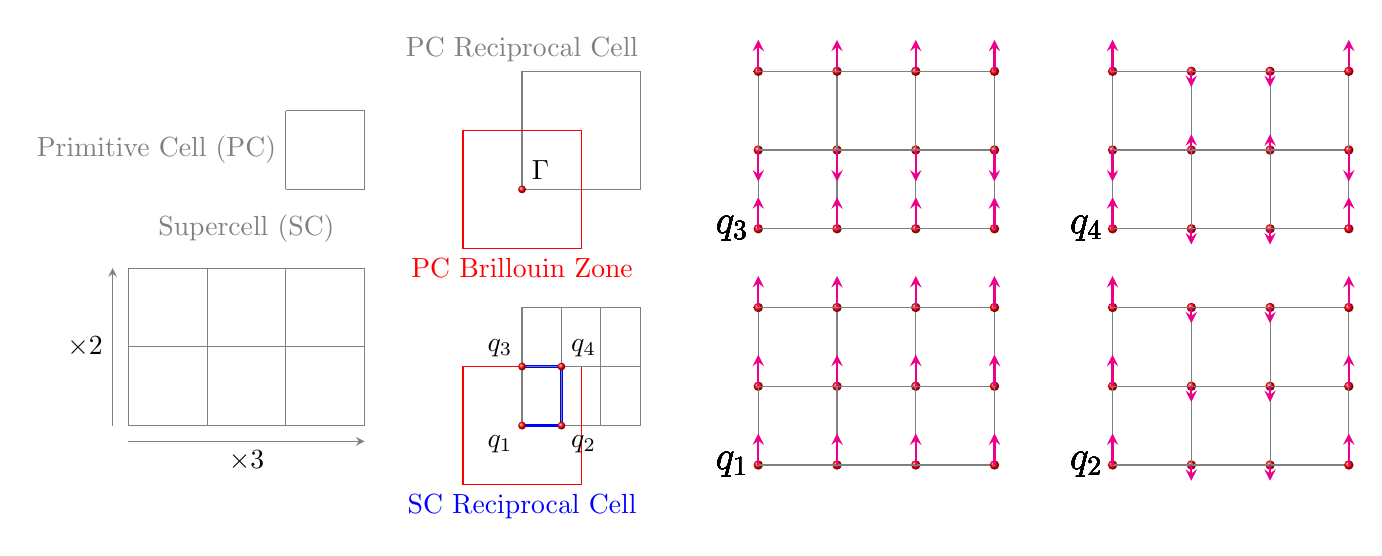
\begin{tikzpicture}
            % the real-space cell
            \draw[help lines, thin] (0, 0) grid +(1, 1);
            \draw[help lines, thin] (-2, -3) grid +(3, 2);
            \draw[->, >=stealth, thin, draw=gray]
            (-2, -3.2) --
            node[pos=0.5, below, anchor=north] {$\times 3$}
            (1, -3.2);
            \draw[->, >=stealth, thin, draw=gray]
            (-2.2, -3.0) --
            node[pos=0.5, left, anchor=east] {$\times 2$}
            (-2.2, -1.0);

            % the primitive BZ
            \draw[help lines, thin] (3.0, 0.0) rectangle +(1.5, 1.5);
            \draw[help lines, thin, draw=red] (2.25, -0.75) rectangle +(1.5, 1.5);

            % supercell BZ
            \draw[help lines, thin] (3.0, -3.0) rectangle +(1.5, 1.5);
            \draw[help lines, thin, draw=red] (2.25, -3.75) rectangle +(1.5, 1.5);
            \draw[help lines, line width=1pt, draw=blue] (3.0, -3.0) rectangle +(0.5, 0.75);

            \draw[thin, draw=gray] (3.0, -2.25) -- (4.5, -2.25);
            \foreach \i in {0, 1, 2, 3}{
            \draw[thin, draw=gray] (3.0 + \i * 0.5, -3) -- (3.0 + \i * 0.5, -1.5);
            }

            \node[align=right, anchor=east, gray] at (0.0, 0.5) {Primitive Cell (PC)};
            \node[align=center, anchor=center, gray] at (-0.5, -0.5) {Supercell (SC)};
            \node[align=center, anchor=center, red] at (3.0, -1.0) {PC Brillouin Zone};
            \node[align=center, anchor=south, gray] at (3.0, 1.5) {PC Reciprocal Cell};
            \node[align=center, anchor=north, blue] at (3.0, -3.75) {SC Reciprocal Cell};

            \shade[ball color=red] (3.0, 0.0) circle (0.05);
            \node[anchor=south west, align=left] at (3.0, 0.0) {$\Gamma$};

            \shade[ball color=red] (3.0, -3.0) circle (0.05);
            \node[anchor=north east, align=center] at (3.0, -3.0) {$\large q_1$};

            \shade[ball color=red] (3.0+1./2, -3.0) circle (0.05);
            \node[anchor=north west, align=center] at (3.0+1./2, -3.0) {$\large q_2$};

            \shade[ball color=red] (3.0, -2.25) circle (0.05);
            \node[anchor=south east, align=center] at (3.0, -2.25) {$\large q_3$};

            \shade[ball color=red] (3.0+1./2, -2.25) circle (0.05);
            \node[anchor=south west, align=center] at (3.0+1./2, -2.25) {$\large q_4$};

            \foreach \x/\y/\l in {6/-3.5/$q_1$, 6/-0.5/$q_3$, 10.5/-3.5/$q_2$, 10.5/-0.5/$q_4$}{
            \foreach \i in {0,1,2,3}{
                \foreach \j in {0,1,2}{
                \draw[thin, draw=gray] (\i + \x, 0 + \y) -- (\i + \x, 2 + \y);
                \draw[thin, draw=gray] (0 + \x, \j + \y) -- (3 + \x, \j + \y);
                \shade[ball color=red] (\x + \i, \y + \j) circle (0.06);
                \node[left=0.04, anchor=east] at (\x, \y) {\Large \l};
                }
            }
            }

            \foreach \x/\y/\qx/\qy in {6/-3.5/0/0, 6/-0.5/0/0.5, 10.5/-3.5/0.333333333/0, 10.5/-0.5/0.333333333/0.5}{
            \foreach \i in {0,1,2,3}{
                \foreach \j in {0,1,2}{
                \pgfmathparse{0.4 * cos((\i *\qx * 2 * pi + \j * \qy * 2 * pi) r)}
                \let \A = \pgfmathresult
                \draw[->, >=stealth, thick, magenta] (\x+\i, \y+\j) -- ++(0.0, \A);
                }
            }
            }
        \end{tikzpicture}
        }
        \end{center}

    \item $D_{s\alpha, t\beta}(\boldsymbol{q})$
        \tikz\draw[->, >=stealth, blue, line width=0.5pt]
        (0, 0) -- node [above] {FT} (1.0, 0.0);
        $C_{s\alpha, t\beta}^{0, l}$
        \tikz\draw[->, >=stealth, blue, line width=0.5pt]
        (0, 0) -- node [above] {Eq.~\ref{eq:dynmat_howto}} (1.0, 0.0);
        $D_{s\alpha, t\beta}(\boldsymbol{k})$
    \end{itemize}

    \break
    
  \item Lineare response theory --- density functional perturbation theory
    \begin{itemize}
    \setbeamercolor{local structure}{fg=red}
    \item Can calculate $D_{s\alpha, t\beta}(\boldsymbol{q})$ at arbitrary
      $\boldsymbol{q}$.
      
    \item $D_{s\alpha, t\beta}(\boldsymbol{q})$ is periodic in reciprocal space: 
    $D_{s\alpha, t\beta}(\boldsymbol{q + G}) = D_{s\alpha, t\beta}(\boldsymbol{q})$
    %   \tikz[baseline=(current bounding box.west)]
    %     \draw[->, >=stealth, blue, line width=0.5pt]
    %     (0, 0) --
    %     node [above] {FT}
    %     node [below] {Uniform $q$-mesh}(2.5, 0.0);
    % $C_{s\alpha, t\beta}^{0, l}$
    %   \tikz[baseline=(current bounding box.west)]
    %     \draw[->, >=stealth, blue, line width=0.5pt]
    %     (0, 0) --
    %     node [above] {Eq.~\ref{eq:dynmat_howto}}
    %     node [below] {Arbitrary $\boldsymbol{q}$} (1.5, 0.0);
    % $D_{s\alpha, t\beta}(\boldsymbol{k})$
    
    \medskip
    \begin{center}
      \resizebox{0.75\textwidth}{!}
      {
      \begin{tikzpicture}
        \draw[draw=red, line width=1pt] (-1, -1) rectangle +(2, 2);
        % \draw[draw=blue, line width=0.5pt, step=0.5] (-1, -1) grid (1, 1);
        \foreach \i in {1, 2, 3}{
            \foreach \j in {1, 2, 3}{
              \draw[blue!50, thin] (2 * \i / 4 - 1, -1) -- ++(0.0, 2.0);
              \draw[blue!50, thin] (-1, 2 * \j / 4 - 1) -- ++(2.0, 0.0);
             }
        }
        
        \draw[-{Stealth[length=6pt, open]}, thick, gray] (1.1, 0.0) --
        node[above, pos=0.5] {FT}
        (2.9, 0.0);

        % \draw[draw=black, line width=0.5pt, step=0.5] (3, -1.4999) grid (6, 1.5001);
        \foreach \i in {0,1,...,4}{
            \foreach \j in {0,1,...,4}{
              \draw[gray, thin] (\i * 0.8 + 3, -1.6) -- ++(0.0, 3.2);
              \draw[gray, thin] (3, \j * 0.8 - 1.6) -- ++(3.2, 0.0);
             }
        }

        \draw[-{Stealth[length=6pt, open]}, thick, gray] (6.3, 0.0) --
        node [above, pos=0.5] {Eq.~\ref{eq:dynmat_howto}}
        (7.9, 0.0);

        \draw[draw=red, line width=1pt] (8, -1) rectangle +(2, 2);
        % \draw[draw=blue, line width=0.5pt, step=0.25] (8, -1) grid +(2, 2);
        \foreach \i in {1,2,...,7}{
            \foreach \j in {1,2,...,7}{
              \draw[blue!50, thin] (8 + 2 * \i / 8, -1) -- ++(0.0, 2.0);
              \draw[blue!50, thin] (8, 2 * \j / 8 - 1)  -- ++(2.0, 0.0);
             }
        }

        \node[align=center, anchor=north, below=3pt, red] at (0.0, -1.0) {Primitive Cell BZ};
        \node[align=center, anchor=north, below=3pt, gray] at (4.6, -1.6) {Real-space Lattice};
        \node[align=center, anchor=south, above=3pt] at (0.0, 1.0) {
          $D_{s\alpha, t\beta}(\boldsymbol{q})$
        };
        \node[align=center, anchor=south west] at (0.0, 0.0) {
          $\Gamma$
        };
        \shade[ball color=red] (0.0, 0.0) circle (0.06);

        \draw[->, >=stealth, black] (4.6, 0.0) -- (5.4, 0.8);
        \node[align=center, anchor=south] at (5.4, 0.8) {
          $C^{0, l}_{s\alpha, t\beta}$
        };

        \node[align=center, anchor=south, above=3pt] at (9.0, 1.0) {
          $D_{s\alpha, t\beta}(\boldsymbol{q}')$
        };
        \draw[black, thick] (9.0, 0.0) -- ++(1.0, 1.0) -- ++(0.0, -1.0) -- cycle;

      \end{tikzpicture}
      }
    \end{center}
    \end{itemize}
  \end{enumerate}
\end{frame}

%%% Local Variables:
%%% mode: latex
%%% TeX-master: t
%%% End:
